% !TEX encoding = UTF-8 Unicode

\section{Descrição Informal da Linguagem}
\label{sec:desc-informal}

O programa é composto por quatro partes, explicadas abaixo de forma 
simplificada, pois a linguagem será definida de forma completa nas seções~\ref{sec:bnf} e~\ref{sec:wirth} nas notações \verb!BNF! e
\verb!Wirth!, respectivamente:

\begin{itemize}
    \item Definição do programa:
            
            Um programa em \verb!czar! possui em ordem obrigatória, a
            importação de bibliotecas, declaração de variáveis globais,
            definição de funções e procedimentos. O programa deve terminar
            obrigatoriamente pela declaração da função principal \verb!main!.

        \begin{itemize}
            \item \verb$PROGRAM = IMPORTS DECLS_GLOBAIS DEF_PROCS_FUNCS DEF_MAIN.$
        \end{itemize}
    \item Inclusão de bibliotecas:
        \begin{itemize}
            \item \verb$IMPORTS = { `<' IDENT `>' }.$
        \end{itemize}
    \item Declaração de tipos, variáveis e constantes de escopo global:
        \begin{itemize}
            \item \verb$DECLS_GLOBAIS = { DEF_TIPO | DECL }.$
            \item \verb$DEF_TIPO = `struct' IDENT `{' { DECL } `}'.$
            \item \verb$DECL = [ `const' ] TIPO IDENT [ `=' EXPR ]$\\
                    \verb${ `,' IDENT [ `=' EXPR ] } `;'.$
        \end{itemize}
    \item Definição dos procedimentos e funções do programa, 
        As funções não devem incluir o procedimento principal (chamado
        \verb!main!). Estas também possuem retorno final único e obrigatório. 
        \begin{itemize}
            \item \verb$DEF_PROCS_FUNCS = { PROC | FUNC }.$
            \item \verb$FUNC = TIPO IDENT LIST_PARAMS$\\
                    \verb$`{' { INSTR_SEM_RET } "return" EXPR [ ";" ] `}'.$
            \item \verb$PROC = `void' IDENT LIST_PARAMS `{' { INSTR_SEM_RET } `}'.$
            \item \verb$LIST_PARAMS = `(' [ [ `ref' ] TIPO IDENT ]$\\
                    \verb${ `,' [ `ref' ] TIPO IDENT } `)'.$
        \end{itemize}
    \item Definição do procedimento principal (chamado \verb!main!):
            
            Não existe
            passagem explícita de parâmetros para a função \verb!main!, ou seja,
            a passagem de valores para a mesma deve ocorrer por meio de
            arquivos ou pela utilização de uma função incluida por alguma
            biblioteca \emph{built-in} a ser feita, permitindo o acesso dos
            parâmetros em todas as partes do código. 
        \begin{itemize}
            \item \verb$DEF_MAIN = `main' `(' `)' `{' [ BLOCO ] `}'.$
        \end{itemize}
\end{itemize}

\section{Descrição da Linguagem em BNF}
\label{sec:bnf}

Apesar de termos visto em aula que a sintaxe BNF não costuma ter os não-terminais explicitados entre aspas, prefirimos colocar aspas simples para facilitar a leitura, que também é uma forma válida de sintaxe BNF\footnote{Ver http://www.cs.man.ac.uk/~pjj/bnf/bnf.html}.

\begin{lstlisting}[frame=single,numbers=left,breaklines=true,mathescape=true>,basicstyle=\ttfamily\scriptsize]
<PROGRAM>            ::= <IMPORTS> <DECLS_GLOBAIS> <DEF_PROCS_FUNCS> <DEF_MAIN>

<IMPORTS>            ::= $\epsilon$
                       | '<' <IDENT> '>' <IMPORTS>

<DECLS_GLOBAIS>      ::= $\epsilon$
                       | <DEF_TIPO> <DECLS_GLOBAIS>
                       | <DECL_CONST> <DECLS_GLOBAIS>
                       | <DECL_VAR> <DECLS_GLOBAIS>  

<DEF_TIPO>           ::= 'struct' <IDENT> '{' <DEF_INSTR_TIPO> '}'

<DEF_INSTR_TIPO>     ::= $\epsilon$
                       | <DECL_CONST>
                       | <DECL_VAR>

<DECL_CONST>         ::= 'const' <DECL_VAR>

<DECL_VAR>           ::= <TIPO> <IDENT> <DECL_VAR_CONT> ';'
                       | <TIPO> <IDENT> '=' <EXPR> <DECL_VAR_CONT> ';'

<DECL_VAR_CONT>      ::= $\epsilon$
                       | ',' <IDENT> <DECL_VAR_CONT>
                       | ',' <IDENT> '=' <EXPR> <DECL_VAR_CONT>

<DEF_PROCS_FUNCS>    ::= $\epsilon$
                       | <PROC> <DEF_PROCS_FUNCS>
                       | <FUNC> <DEF_PROCS_FUNCS>

<FUNC>               ::= <TIPO> <IDENT> <LIST_PARAMS> '{' <INSTRUCOES> 'return' <EXPR> '}'
                       | <TIPO> <IDENT> <LIST_PARAMS> '{' <INSTRUCOES> 'return' <EXPR> ';' '}'

<PROC>               ::= 'void' <IDENT> <LIST_PARAMS> '{' <INSTRUCOES> '}'

<INSTRUCOES>         ::= $\epsilon$
                       | <INSTR_SEM_RET> <INSTRUCOES>

<LIST_PARAMS>        ::= '(' ')'
                       | '(' <TIPO> <IDENT> <LIST_PARAMS_CONT> ')'
                       | '(' 'ref' <TIPO> <IDENT> <LIST_PARAMS_CONT> ')'

<LIST_PARAMS_CONT>   ::= $\epsilon$
                       | ',' <TIPO> <IDENT> <LIST_PARAMS_CONT>
                       | ',' 'ref' <TIPO> <IDENT> <LIST_PARAMS_CONT>

<DEF_MAIN>           ::= 'main' '(' ')' '{' <INSTRUCOES> '}'

<INSTR_SEM_RET>      ::= <DECL_VAR>
                       | <ATRIB>
                       | <PROC_CALL>
                       | <FLOW_CONTROL>

<ATRIB>              ::= <ATRIB_SEM_PV> ';'

<ATRIB_SEM_PV>       ::= <VARIDENT> <OPER_ATRIB> <EXPR> <ATRIB_SEM_PV_CONT>

<ATRIB_SEM_PV_CONT>  ::= $\epsilon$
                       | ',' <VARIDENT> <OPER_ATRIB> <EXPR> <ATRIB_SEM_PV_CONT>

<PROC_CALL>          ::= <IDENT> '(' ')' ';'
                       | <IDENT> '(' <EXPR> <PROC_CALL_CONT> ')' ';'

<PROC_CALL_CONT>     ::= $\epsilon$
                       | ',' <EXPR> <PROC_CALL_CONT>

<FLOW_CONTROL>       ::= <FOR_CONTROL>
                       | <WHILE_CONTROL>
                       | <IF_CONTROL>

<FOR_CONTROL>        ::= 'for' '(' <DECL_VAR> <COND> ';' <ATRIB_SEM_PV> ')' '{' <INSTRUCOES> '}'

<WHILE_CONTROL>      ::= 'while' '(' <COND> ')' '{' <INSTRUCOES> '}'

<IF_CONTROL>         ::= 'if' '(' <COND> ')' '{' <INSTRUCOES> '}'
                       | 'if' '(' <COND> ')' '{' <INSTRUCOES> '}' 'else' '{' <INSTRUCOES> '}'

<TIPO>               ::= <IDENT> <TIPO_CONT>

<TIPO_CONT>          ::= $\epsilon$
                       | '[' <INT> ']' <TIPO_CONT>

<IDENT_COLCHETES>    ::= <IDENT> <IDENT_COLCH_CONT>

<IDENT_COLCH_CONT>   ::= $\epsilon$
                       | '[' <EXPR> ']' <IDENT_COLCH_CONT>

<VARIDENT>           ::= <IDENT_COLCHETES> <VARIDENT_CONT>

<VARIDENT_CONT>      ::= $\epsilon$
                       | '.' <VARIDENT> <VARIDENT_CONT>

<FUNCTION_CALL>      ::= <IDENT> '(' ')'
                       | <IDENT> '(' <EXPR> <FUNCTION_CALL_CONT> ')'

<FUNCTION_CALL_CONT> ::= $\epsilon$
                       | ',' <EXPR> <FUNCTION_CALL_CONT>

<COND>               ::= <COND_TERM> 
                       | <COND_TERM> <OPER_BOOL> <COND_TERM>

<COND_TERM>          ::= '(' <COND> ')' 
                       | <ATOMO_COND> 
                       | <ATOMO_COND> <OPER_COMP> <COND_TERM>

<ATOMO_COND>         ::= <VARIDENT> 
                       | 'true'
                       | 'false'
                       | <INT> 
                       | 'not' <ATOMO_COND>

<OPER_ATRIB>         ::= '+=' 
                       | '-=' 
                       | '*=' 
                       | '/=' 
                       | '%=' 
                       | '=='

<OPER_BOOL>          ::= 'and' 
                       | 'or'

<OPER_COMP>          ::= '==' 
                       | '!=' 
                       | '<=' 
                       | '>='

<OPER_ARIT>          ::= '+' 
                       | '-'

<OPER_TERM>          ::= '*' 
                       | '/' 
                       | '%'

<EXPR>               ::= <TERM> 
                       | <TERM> <OPER_ARIT_TERM_ARR>
                       | <OPER_ARIT_TERM_ARR>

<OPER_ARIT_TERM_ARR> ::= <OPER_ARIT> <TERM>
                       | <OPER_ARIT> <TERM> <OPER_ARIT_TERM_ARR>

<TERM>               ::= '(' <EXPR> ')'
                       | <ATOMO>
                       | <ATOMO> <OPER_TERM_ATOMO_ARR>

<OPER_TERM_ATOMO_ARR>::= <OPER_TERM> <ATOMO>
                       | <OPER_TERM> <ATOMO> <OPER_TERM_ATOMO_ARR>

<ATOMO>              ::= <FUNCTION_CALL>
                       | <OPER_ARIT> <FUNCTION_CALL>
                       | <INT>
                       | <OPER_ARIT> <INT>
                       | <STRING>
                       | <CHAR>
                       | <FLOAT>
                       | <OPER_ARIT> <FLOAT>
                       | <BOOL>
                       | <VARIDENT>
                       | <OPER_ARIT> <VARIDENT>
\end{lstlisting}

\section{Descrição da Linguagem em Wirth}
\label{sec:wirth}

\lstinputlisting[frame=single,numbers=left,breaklines=true,basicstyle=\ttfamily\scriptsize]{files/WIRTH.txt}

\section{Diagrama de Sintaxe da Linguagem}
\label{sec:diagrama-sintaxe}

\begin{figure}[H]
	\centering 
	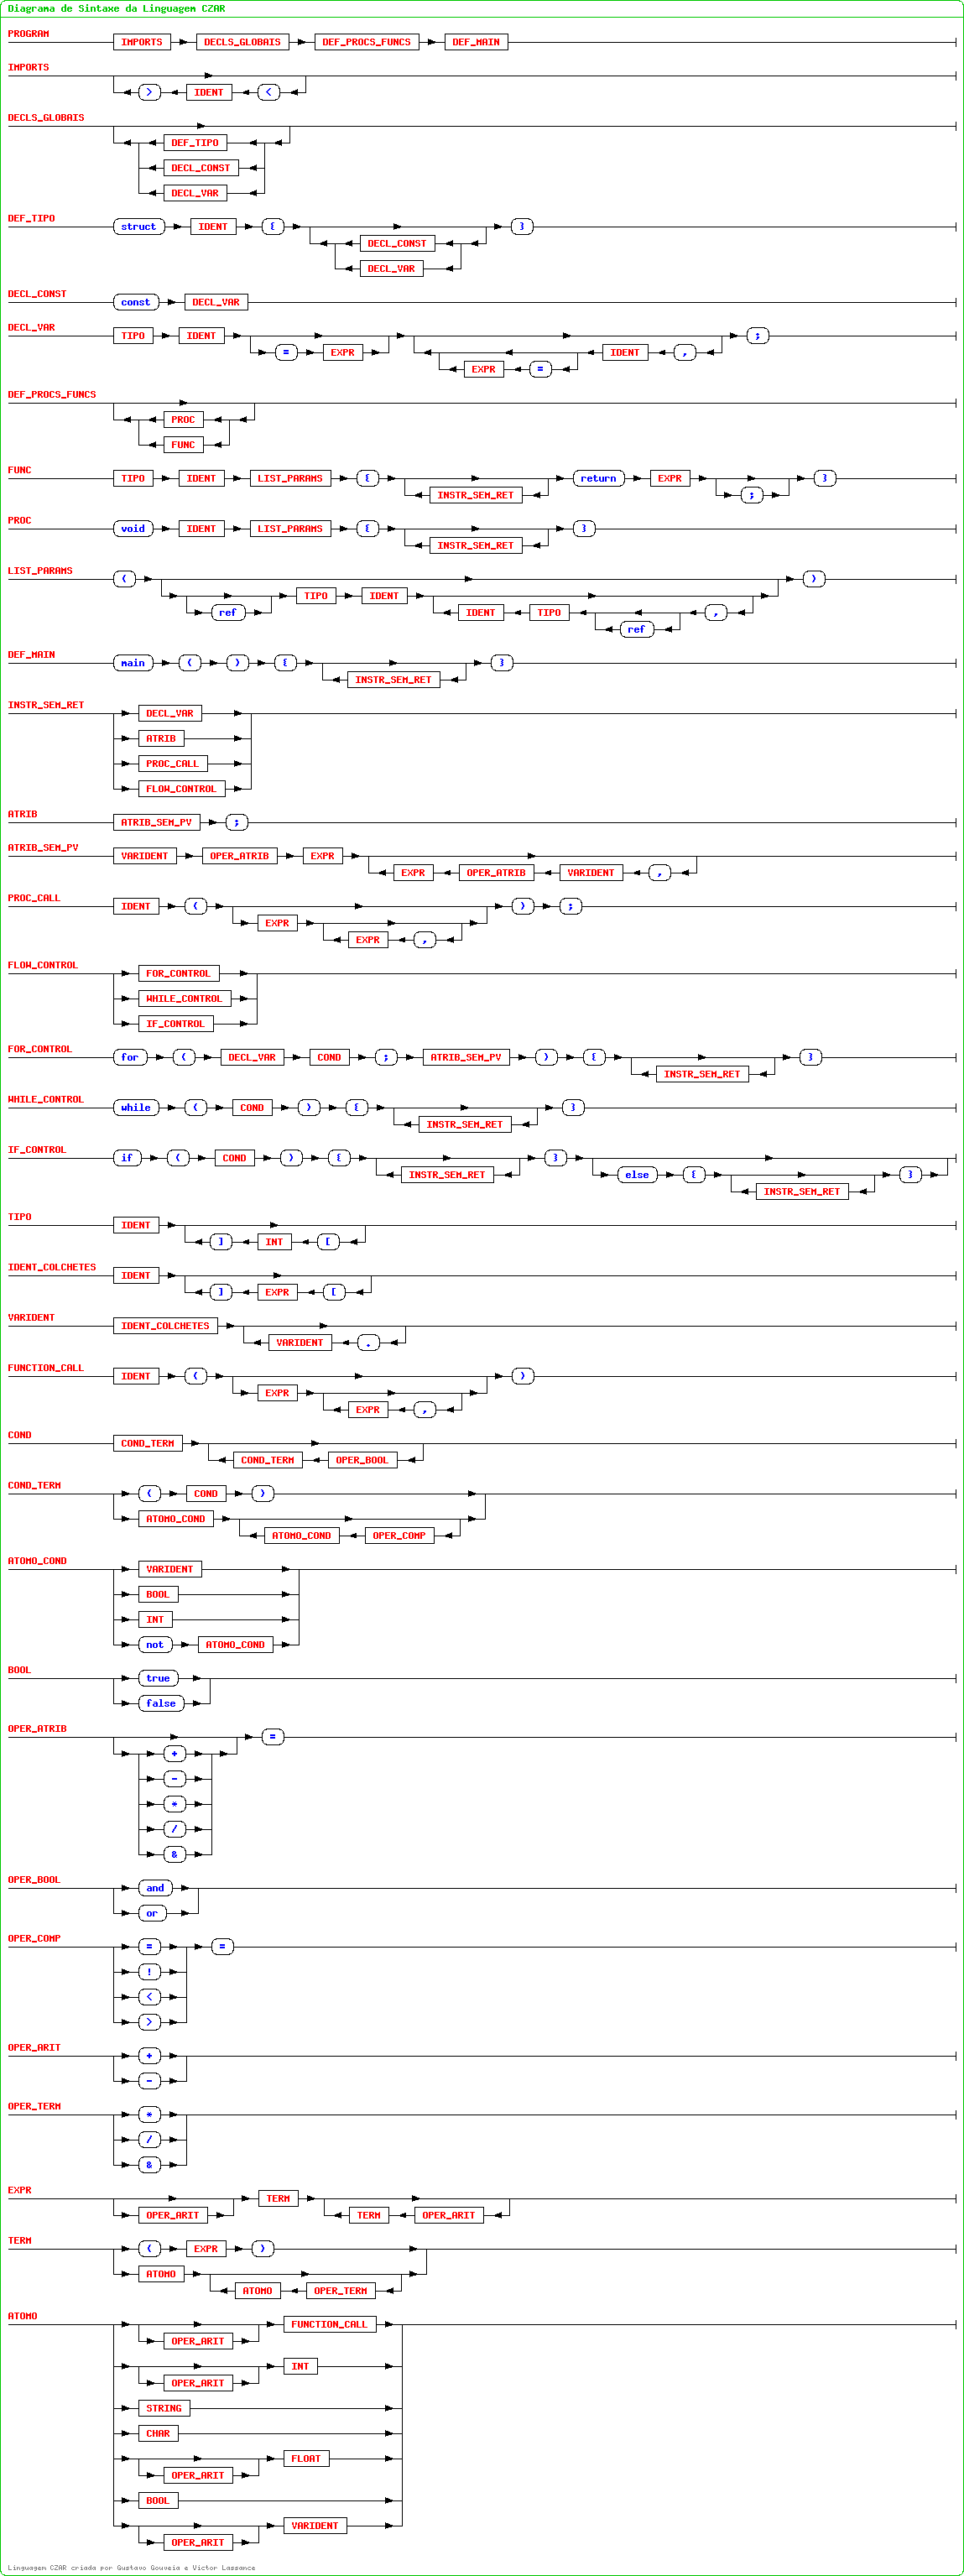
\includegraphics[width=\textwidth, clip, trim=0 1635px 0 0]{images/diagrama-sintaxe.png}  
	\label{fig:diagrama-sintaxe-1}
\end{figure}

\begin{figure}
	\centering 
	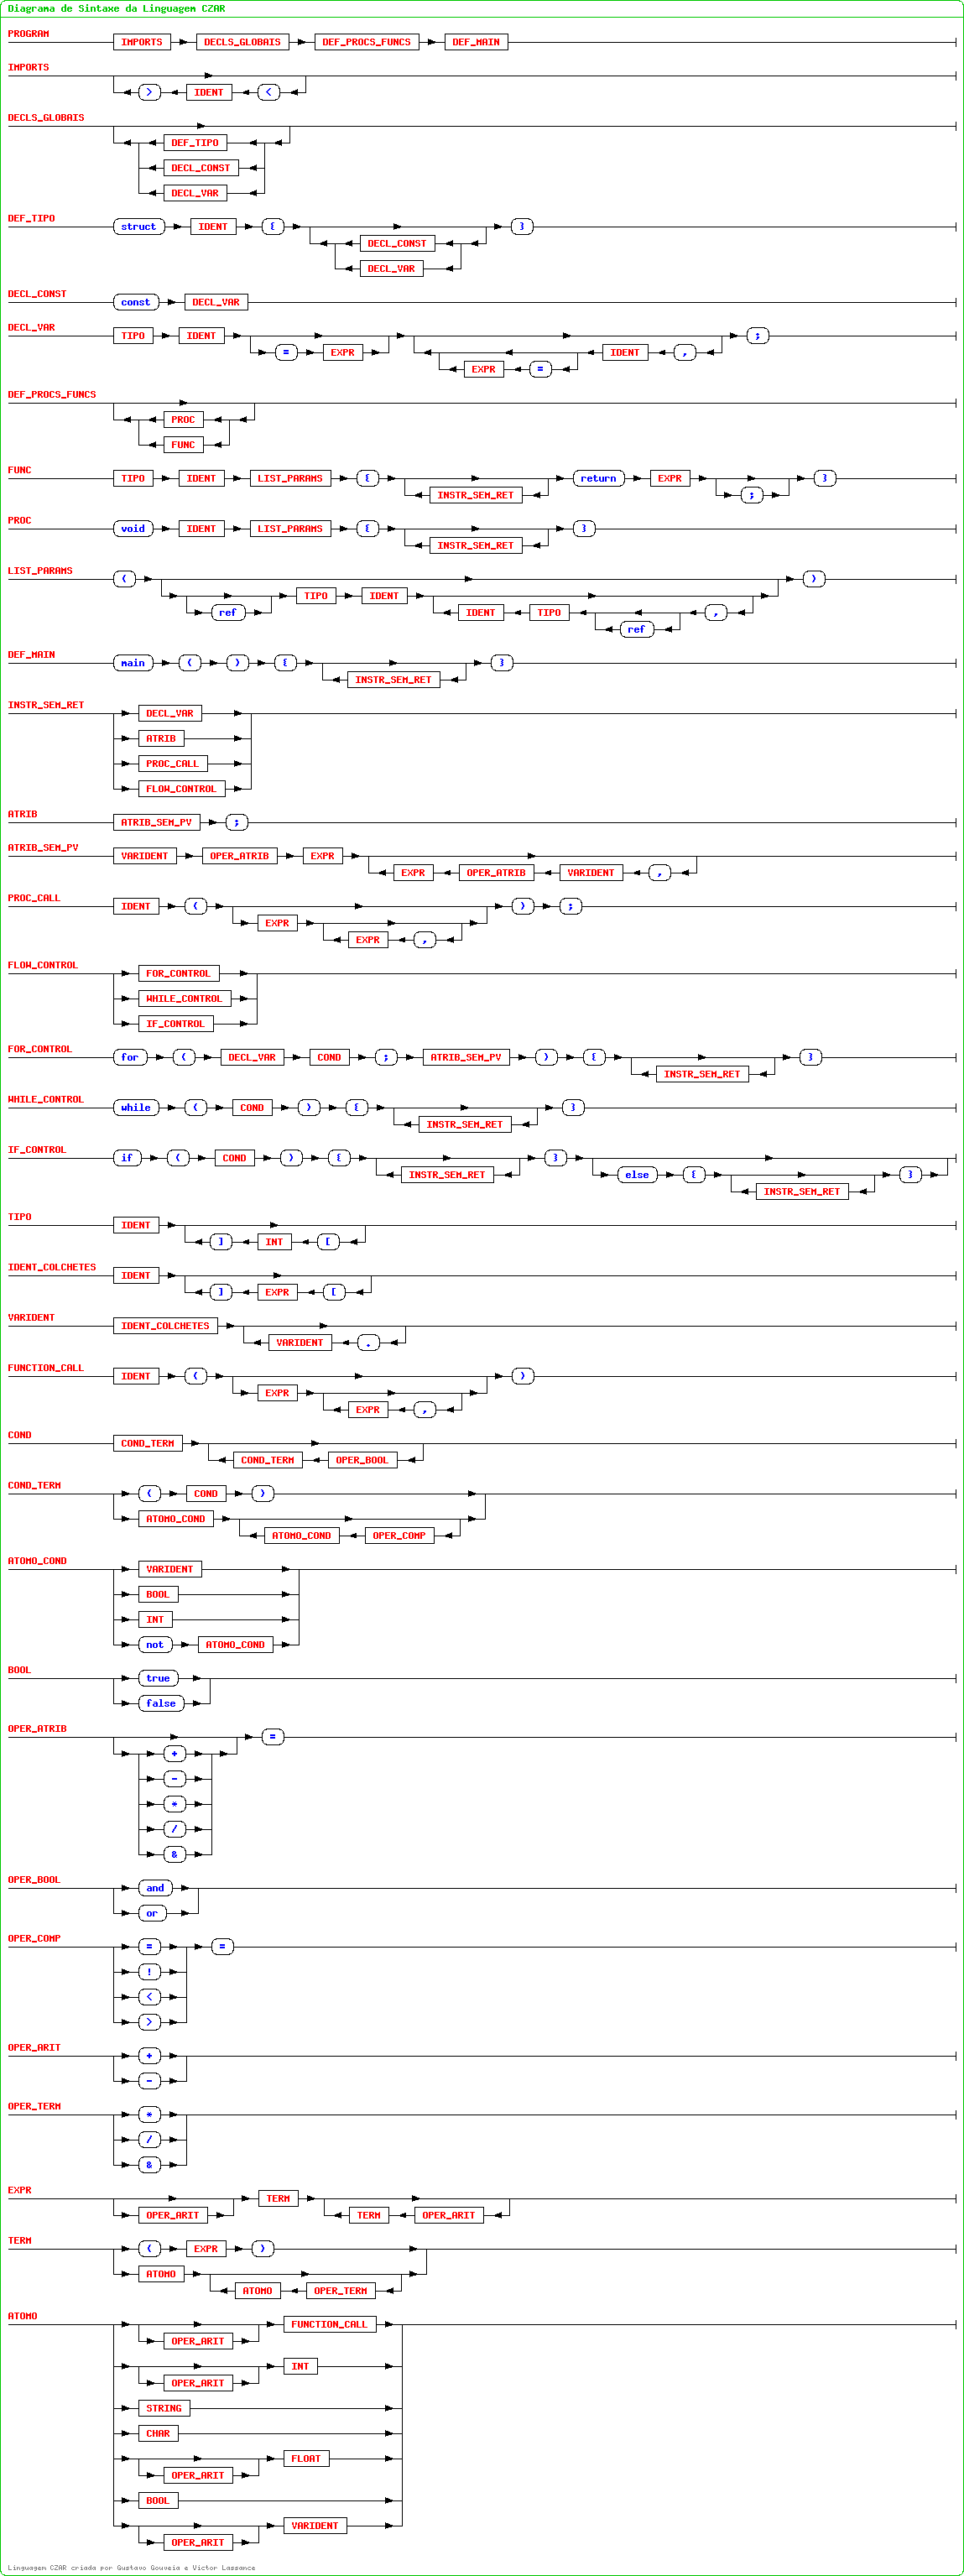
\includegraphics[width=\textwidth, clip, trim=0 0 0 1435px]{images/diagrama-sintaxe.png} 
	\caption{Diagrama de Sintaxe da Linguagem CZAR}
	\label{fig:diagrama-sintaxe-2}
\end{figure}
